\subsection{Virtual Reality}
\label{sec:virtual-reality}
% what is virtual reality?
VR immerses users in an interactive digital environment using a head-mounted display.
The ``ultimate display" as described by Ivan Sutherland is a theoretical human-computer interaction device that simulates a reality that is realistic to the point where a person cannot tell the difference between actual reality and the simulated reality~\cite{Sutherland1965}.
This level of immersion in a completely new world was an appealing idea even before the technological inception of a device that was even remotely capable of achieving it.
The virtual world appears realistic to a human through the use of stereoscopic displays and sound.
Stereoscopic displays present each eye with a different image for the user to experience simulated depth.
Also, gives the user the ability to interact with the virtual objects in a realistic way with tactile feedback.
% This includes not just observing the virtual world, 
% The concept VR follows the ideals of the ``ultimate display" has shaped the ideas and ideals for VR technology, where with every iteration of the technology it becomes evermore achievable. 
Since the 1960s, the concept of virtual VR headsets has evolved significantly. 
One of the earliest examples dates back to this era, with Morton Heilig's Telesphere Mask~\cite{Heilig1994} which introduced the notion of a head-mounted display. 
It offered wide vision, a stereoscopic 3D display, and stereo sound; it was later augmented by the introduction of a motion tracking feature in 1961.
Over time, various entities, including NASA, Sega, Nintendo, Apple, and Google, have experimented with VR technology. 
Recent advancements have been marked by Oculus, now owned by Meta, which is releasing affordable VR headsets aimed at mass market consumption, particularly targeting the entertainment sector.
However, VR technology is in the process of being adopted in other industries such as education, retail, transportation, energy, consulting, insurance, healthcare, and sports.

\begin{figure}
    \centering
    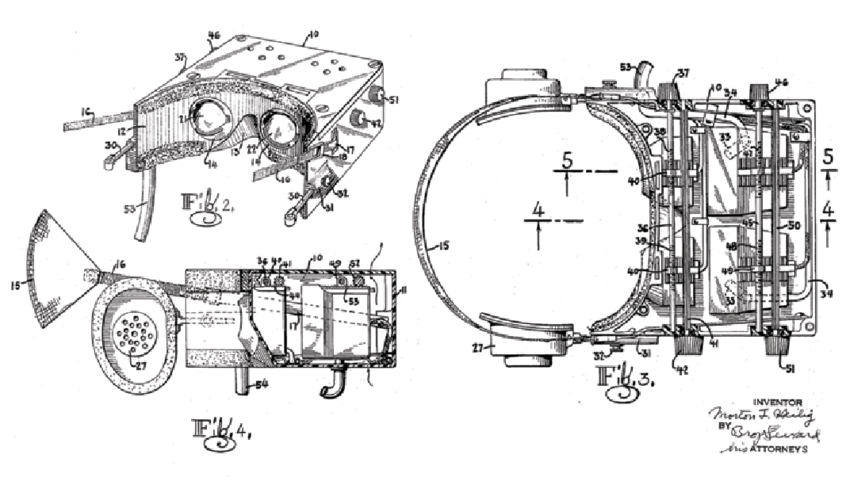
\includegraphics[width=\linewidth]{figures/telesphere-mask.png}
    \caption{Morton Heilig's patent for the Telesphere Mask~\cite{Heilig1994}, note the resemblance to contemporary headset design, such as the Meta Oculus Quest and the Apple Vision Pro.}
    \label{fig:telesphere}
\end{figure}

% what does it do?
%\cite{Wohlgenannt2020} % add othe citations mentioned in this paper
VR uses immersive technology to simulate interactive virtual environments where users feel physically present~\cite{Wohlgenannt2020, Bowman2007}.
This is done through the construction of a real or imagined environment, which blocks the real world from the user.
It also incorporates interaction methods such as controllers and motion tracking for the user to interact with the environment~\cite{Brooks1999, Barfield2000}.

% other VR tecnologies
% augmented reality (AR), augmented virtuality (AV), terms also refered to as mixed reality (MR) superimposes virtual agents over the real world in real-time (added digital information to physical reality)
% the term extended reality (XR) is a term used to refer to all the possible combinations of  real-and-virtual environments and human–machine interactions generated by computer technology and wearables
%  used as a umbrella term for their combined use

\begin{figure}
    \centering
    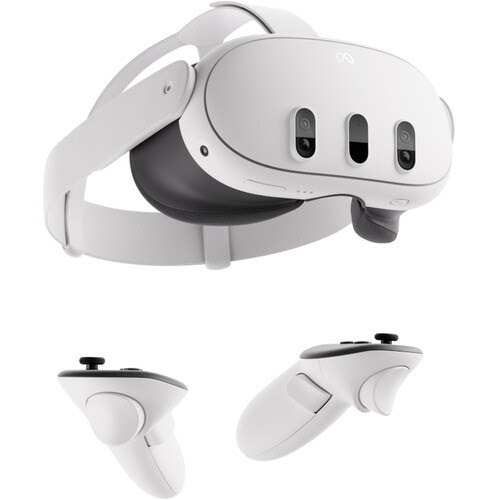
\includegraphics[width=0.6\linewidth]{figures/oculus-quest.jpg}
    \caption{An example of one of the latest iterations of VR technology, Meta's Oculus Quest 2. It can be considered as a extended reality (XR) headset as it can host VR environments while also incorporation augmented reality (AR) features.}
    \label{fig:oculus-quest-2}
\end{figure}

VR experience can be evaluated according to three key properties: presence, interactivity, and immersion~\cite{Walsh2002}.
% presense refers to the sense of physically being somewhere other where someone actually is
Presence refers to the sense of being physically somewhere.
Within a virtual environment, the presence of the user is simulated by capturing their senses, using visual, audio, and tactile simulations~\cite{Sanchez2005}.
% visual, ausio and tactil(haptics) realism is an important factor for presense in a virtual environment
% as well as virtual body representation and body engagement
The feeling of being present in virtual environments arises from the way that a user perceives and processes information from their surroundings, both in their conscious and subconscious environment~\cite{Barfield2000}.
% Some factors which contribute to how present a user feels in a virtual environment are: the virtual environment, communication medium, the individual user, any disturbances from the real world and, the task or tasks which the user performs.
% there are factors which contribute to presense
%   the computer and virtual environment
%   the communication medium
%   the individual
%   disturbances from the real-world environment
%   the task
The sense of presence that a user feels is difficult to quantify, as it can be measured in objective and subjective ways.
Subjective measurement comes from the level of realism in the virtual environment.
As VR technology improves, the level of realism VR headsets are able to display improves with it.
% Subjective measures of presense
%   realism is an essential part of presense in a virtual environment
%   as the technology used in contemporary VR headsets improve so does the realism and sense of presense within the environment
The objective measure of presence observes physical indicators in the user; these indicators include heart rate, dilation of the pupils, blink responses, and muscle tension.
% Objective measures of presense
%  physical indicators in a test subject (Heart rate, pupil dilation, blink responses, and possibly muscle tension)
Some more objective measurements include the extent to which physically reality is excluded from the virtual one, the number of the user's senses that are captured by the virtual reality, the extent of the field of view, the resolution and quality of the displays used, and how the user's body movements match up against their movements in the virtual world~\cite{Sanchez2005, Barfield2000}.
% objectively measurable 
%   inclusiveness - the extent to which reality is exculded
%   extensiveness - the range of sensory modalities
%   surrounding - the size of the feild of view
%   vivedness - the richness, resolution, and quality of the displays
%   matching - the extet to which proprioceptive feedback on body movementsin aligned with display information
% Immersion can be quantifiable judged through the assessment of the inclusively, extensiveness, display size and resolution of display technology~\cite{Barfield2000}.
% The aspect of inclusively refers to how much of the real world is the display able to block out from the vision, extensiveness refers to how many senses the technology encapsulates, such as taste, touch, sight, smell, and hearing.
% The display size judges how panoramic the display is and the resolution refers to the level of resolution or number of pixels on the display.
%   inclusive - the degree to which the stimuli from the real world are excluded from the user
%   extensive - the number of sensory modalities accommodated by the system
%   surroundings - how panoramic the displays are
%   vivid - the resolution of the displays
Interactions in the real world are naturally as good as they could possibly be according to both subjective and objective measurements of presence.
Human senses have specifically adapted for perceiving and interacting in the real world, and therefore it is difficult to simulate the same level of realism digitally.

VR Interactivity refers to how effectively a user can manipulate the virtual environment in real time~\cite{Steuer2000}.
In interactive systems, users have agency and control over various elements within the virtual environment, which allows them to make decisions, perform actions, and influence outcomes with their interactions.
This can range from simple actions like clicking buttons or navigating menus to more complex interactions such as manipulating objects, and altering parameters. 
The level of interactivity correlates with the user's sense of immersion and engagement, as it enables them to influence the environment and participate actively in the experience according to their preferences, goals, and intentions.
% interactivity refers to the extent to which a user can manipulate their environment in real time
Interactivity is a key factor as it affects the level of presence the user feels within the environment and directly influences the user's sense of presence. 
% interactivity can affect the presence the user feels within the environment (body engagement)
 
Immersion in VR is more complicated than presence and interactivity.
% It can be classified as subjective involvement which involves cognitive, emotional, sensory-motor, and spatial immersion.
Immersion can be described as subjective involvement, encompassing various dimensions of a user's experience~\cite{Nilsson2016}. 
However, there are many facets of immersion.
Cognitive immersion manifests when a user engages with the content, experiencing satisfaction and fulfilment upon solving complex problems. 
Emotional immersion occurs when a user become emotionally invested in narrative structures, experiencing highs and lows which come with a story. 
Kinesthetic immersion emerges when users receive immediate feedback on their physical actions, which enhances their sense of presence and agency within the virtual environment. 
% The term distal-attribute describes this phenomenon aptly, it is where an individual creates a mental representation of themselves to include the external and virtual worlds.
% For example, when a tool becomes and extension of an individual's body but it is not physically part of it.
% the phenomenon of individuals creating a mental representation of them selves to include in the external and virtual world.
% eg a tool becomes an extension of your body even though it is physically not
Spatial immersion is experienced as users navigate and perform intricate movements, feeling a sense of spatial presence and immersion within the simulated world. 
These dimensions collectively contribute to a rich and immersive user experience across various interactive platforms and media.
%  immersion can also be classifed as subjective involvement
%   cognitive immersion - users feel when they solve complex problems
%   emotional immersion - users feel when narrative structures unfold
%   sensory-motoric immersion - users feel when they receive feedback on movements
%   spatial immersion - users feel when they perform extensive maneuvers/
The sense of presence relates to the perception of the physical environment and is tightly coupled to how immersed the user feels.
Vice versa, the more immersed the user feels in the virtual environment, the easier it is for them to feel present.

While VR systems offer immersive experiences, they face some downsides, notably simulator sickness. 
This condition is caused by to frame rate drops.
Frame rate is the number of images a display such as a screen can cycle through per second.
The rapid succession of frames on the display is what causes the image on the screen to appear to have motion.
When the frame rate is high, the motion on the display appears smooth; low frame rate makes the motion of the image to appear choppy and unpleasant.
It is this choppy movement on the display which leads to a disconnect between user input and display output, which results in feelings of confusion, dizziness, and nausea for some users. 
% Simulator sickness can easily arise from a poorly designed or poorly performing system.
The level of susceptibility to simulator sickness varies between individuals, but has some dependence on a users experience with VR headsets as well as their natural tolerance to being in a VR environment.
Additionally, as the system's performance declines, the immersive element of the experience diminishes, which highlights the sensitivity of VR experiences to hardware performance. 
Users experience disconnect from the environment when any aspect of presence, interactivity, or immersion is compromised.
% A consequence of this disconnect is that a user may experience simulator sickness.
% Thus, the overall experience of a VR system heavily relies on consistent and high-performance hardware to maintain immersion and prevent adverse effects on users.
% the downsides
% simmulator sickness
% frame rate drop produces a disconnect between the user input and the display output causing a feeling of confusion, dizziness and nausea in some users
% the immsersiv element of the experience breaks down as the performance of the system drops
% the experience of a VR system is dependent on the hardware's performance and is incredible sensitive to drops in performance